\documentclass{article}
\usepackage{graphicx} % Required for inserting images

\title{INDENG 242A Project: Time-Series Application in Stocks}
\author{Xi Chen, Yunhao Liang, Zixin Zhang, Zhiming Fan}
\date{December 2024}

\begin{document}

\maketitle

\section{Introduction}
In this project, our aim is to develop an equally weighted portfolio using log-returns of S\&P 500 and Nikkei 225 indices, two well-known stock indices. We determine the risk value (VaR) at the confidence levels 99\% and 95\%.  The VaR estimation is conducted through Monte Carlo Simulations, leveraging Copula theory. 
The project report provides a detailed workflow, from data analysis to model formulation and computation. This study demonstrates the application of Copula-based simulations in risk management and portfolio analysis.

\subsection{Data Processing}
The data is loaded from yahoo finance website and exported as the file '\textit{SP500\_N225.csv}'. For S\&P 500 index, the columns named \textit{Date, Open, High, Low, Close,} \textit{Adj.Close} represents the weekly data. For Nikkei 225 index, the columns named \textit{Date.1, Open.1, High.1, Low.1, Close.1, and Adj.Close.1} represents the weekly data. \\
\\
The data set includes 1,302 weekly observations that span from January 1, 2000, to December 7, 2024. We then compute the weekly log-returns for both indices by taking the natural logarithm of the ratio of the current price to the previous price using the formula \begin{equation}
    r = \log \frac{p_t}{p_{t-1}}.
    \label{eq:log_return}
\end{equation}

\subsection{Exploratory Data Analysis}
We start our exploratory data analysis by plotting the time series of weekly log-returns for the two stock indices.\\
\\
Figures 1 and 2 show the weekly log-returns for the S\&P 500 and Nikkei 225, respectively. It is evident that the log-returns for both indices do not exhibit stable behavior over time. Periods such as week 450 and week 1050 reveal noticeable clusters of volatility, indicative of time-varying conditional mean and variance. \\
\\
Table 1 presents the descriptive statistics of the log-returns. For the S\&P 500, the mean and standard deviation are 0.00096 and 0.025, respectively. The mean log-returns of the Nikkei 225 are 0.00049 with a standard deviation of 0.030. This indicates that while the S\&P 500 exhibits higher average log-returns, its variability is slightly lower than that of the Nikkei 225. \\
\\
The p-values from the Jarque-Bera test reject the null hypothesis of normality for both indices. This finding is consistent with the observed excess kurtosis and negative skewness, suggesting that the log-returns are not normally distributed. \\
\\
Figures 3 and 4 display the density plots of the log-returns (blue lines) alongside the fitted normal distribution (red lines). Both indices exhibit left-skewness and heavier tails compared to a normal distribution, which indicates a higher likelihood of extreme movements in market prices. To account for this, the student-t distribution will be considered in the subsequent modeling process.

\section{Model Construction}
\subsection{Model Building}
Based on all previous analysis, we choose to consider the potential effect by different conditional mean and variance over time when calculating VaRs.
\\For the two indices, we employed ACF (Autocorrelation Function) and PACF (Partial Autocorrelation Function) plots to verify the existence of autocorrelation of the conditional mean and variance.\\
\\The findings of Figures 5-10 are as follows: 
\textbf{Figure 5:} The first lag of S&P 500 lies outside the 95\% confidence interval.
\textbf{Figure 6:} There are three significant lags (1, 15) observed in the PACF plot for Nikkei 225.
\textbf{Figures 7 \& 10:} The squared log-returns of S&P 500 and Nikkei 225 reveal a gradual decaying trend in the first few lags in the ACF plots. This trend indicates a cluster of volatility (conditional heteroskedasticity) for the two indices, consistent with the Ljung-Box test results.
\textbf{Figure 8:} Nikkei 225 autocorrelations are within the 95\% confidence interval, except for lag 24.
\textbf{Figure 9:} The PACF plot shows significance at lags 20 and 24. All Nikkei 225 autocorrelations, except for lag 24, fall within the 95\% confidence interval. The PACF highlights lags 20 and 24.\\ 
\\Based on the Ljung-Box test, ACF, and PACF results, we chose an ARMA-GARCH model for the S\&P 500 log returns and a GARCH model for the Nikkei 225.\\
\\We selected the Skew Student t-distribution as the conditional distribution due to its lowest AIC. For the S\&P 500, we tested ARMA(1,0) to ARMA(3,3) combined with GARCH(1,1) to GARCH(3,3). While ARMA(3,3)-GARCH(1,1) had the lowest AIC and ARMA(1,1)-GARCH(1,1) the lowest BIC, only ARMA(1,0)-GARCH(1,1) passed the Ljung-Box test, making it the most reliable choice.\\
\\For the Nikkei 225, the autocorrelation test indicated no first-moment serial correlation, so we focused on GARCH models. The GARCH(1,1) model had the lowest AIC and was selected as the best fit.\\
\\Ultimately, we used the AR(1)-GARCH(1,1) model for the S\&P 500 and the GARCH(1,1) model for the Nikkei 225.\\

\subsection{Model Checking}
We assessed model adequacy using the Ljung-Box test on residuals and squared residuals. Table 3 shows that all p-values exceed 0.05, indicating the models are a good fit. ACF plots for residuals and squared residuals confirm that most lags fall within the 95\% confidence interval, suggesting autocorrelation in conditional mean and variance has been removed. \\
\\In Figure 11 for the S&P 500, a small peak at lag 1 appears in the ACF plot, hinting at potential autocorrelation in residuals. Despite testing models from ARMA(0,0)-GARCH(1,1) to ARMA(3,3)-GARCH(3,3), this persists. Ljung-Box results, however, support the model's reliability. Higher-order models were avoided due to computational complexity. Thus, we proceed with ARMA(1,0)-GARCH(1,1) for the S&P 500. Future research could explore alternative methods or seasonal adjustments.\\
\\Residuals reflect unexplained movements in stock indices beyond historical trends and volatility. To analyze these components, we use a Copula model (Bivariate Copula: Survival BB1, par = 0.13, par2 = 1.46, tau = 0.36) to evaluate correlations between the S&P 500 and Nikkei 225. The Probability Integral Transform (PIT) is applied to residuals to ensure uniformity, with PIT plots provided below.\\

\section{Model Evaluation: Value-at-Risk Using Monte Carlo Simulation}
To evaluate our model, one of the best way is to take simulations to see what happens for large scale of situations. The following plots demonstrate the observed Copula and simulated Copula. Uniform marginal distributions are indicated in the left plot, representing a positive correlation between two stocks and a clustering behavior at the lower left and upper right. The right simulation plot matches all characteristics in the left well: positive correlations, clustering, which means it is a valid way describing real world financial market. \\
\\
Applying inverse possibility integral allows us to transform simulated residuals back to their original distribution. GARCH model can be used again for the simulated residuals. Then  the original log-returns and simulated log-returns of the two stock indices can be shown in the following graphs. This means that the simulated pattern is largely dependent on the observed one.\\
\\
Finally, an equally weighted portfolio is constructed and the Value-at-Risk of 99\% and 95\% confident interval are taken to give a direct evaluation of our model. From table we can conlude that in 99\% cases we will not lose more than \$74,690, and a loss \$37,070 will not appear in 95\% case.

\section{Conclusion}
In this project, we applied machine learning techniques to analyze time series data for portfolio risk management, focusing on the S\&P 500 and Nikkei 225 indices. By using ARMA-GARCH models and Copula-based Monte Carlo simulations, we constructed a robust framework for estimating the Value-at-Risk (VaR) of an equally weighted portfolio. \\
\\
Our analysis revealed the importance of addressing volatility clustering and dependence structures between assets, which are critical in accurately estimating risk measures. Using Copula theory, we modeled the joint distribution of the indices, allowing us to simulate portfolio returns and compute VaR at the confidence levels 99\% and 95\%. \\
\\
The problem we solved was to estimate portfolio risks, providing critical insight for financial decision making. The data used consisted of weekly adjusted closing prices for the S\&P 500 and Nikkei 225 indices, processed to compute logarithmic returns. The models demonstrated reliability, validated by diagnostic tests such as the Ljung-Box test, and highlighted the potential for significant losses during volatile periods. \\
\\
Future extensions of this work could integrate additional features, such as macroeconomic indicators, to further refine risk estimation. Exploring advanced machine learning techniques, including deep learning for time series forecasting, could also enhance model accuracy and robustness. Overall, this project provides a strong foundation for applying machine learning methodologies to time series problems in finance, demonstrating their effectiveness in solving complex real-world challenges.

\newpage
\section{Plots \& Tables}

\begin{figure}[htb]
    \centering
    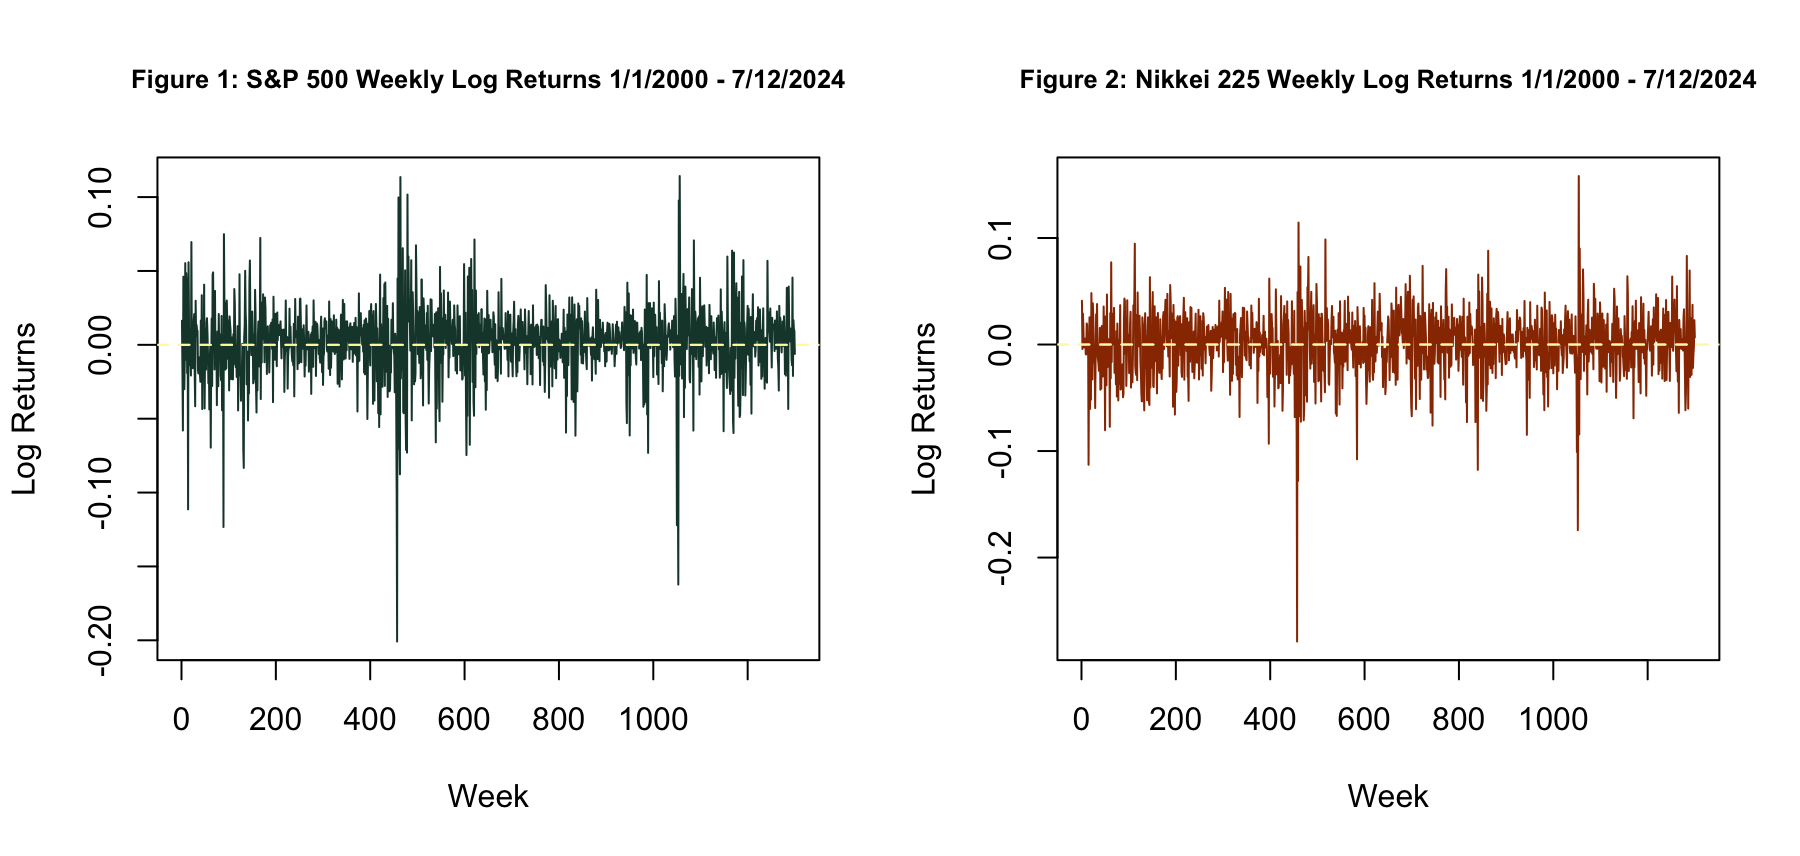
\includegraphics[width=1\linewidth]{WeeklyLogReturns.png}
\end{figure} 
\\
\begin{figure}[htb]
    \centering
    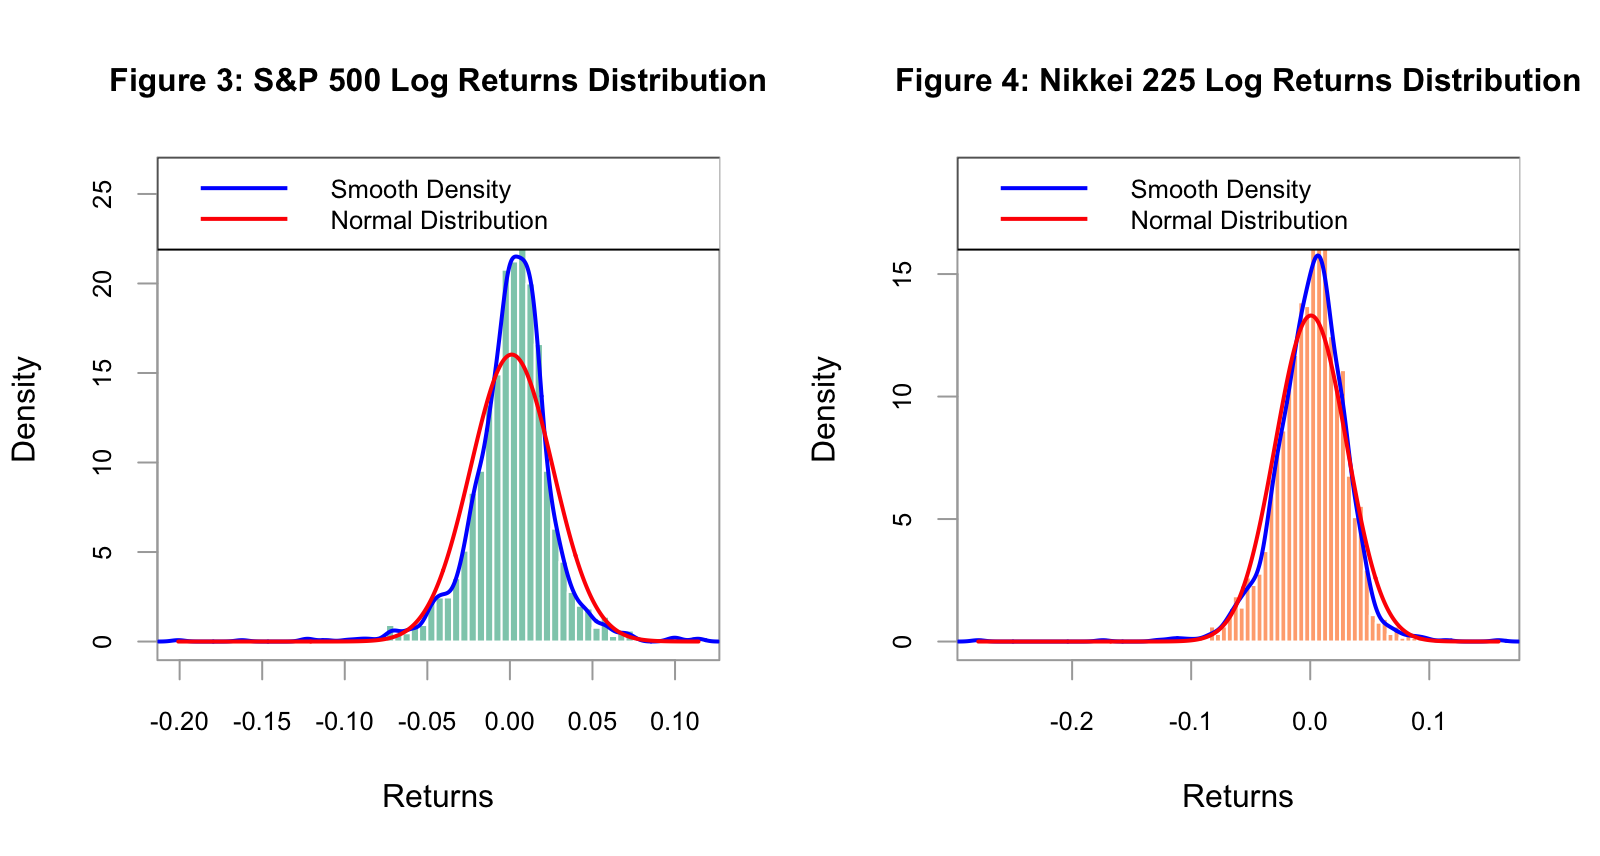
\includegraphics[width=1\linewidth]{Log Returns Distribution.png}
\end{figure}
\begin{figure}[htb]
    \centering
    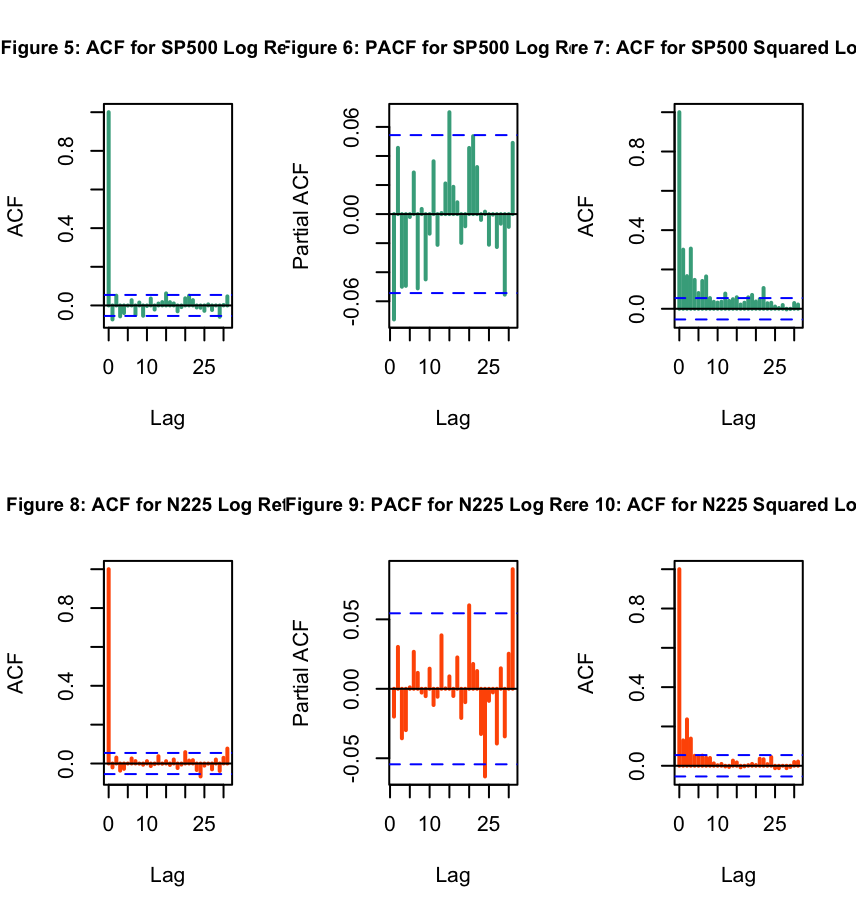
\includegraphics[width=1\linewidth]{Figure 5-10.png}
    \label{fig:enter-label}
\end{figure}

\begin{figure}[htb]
    \centering
    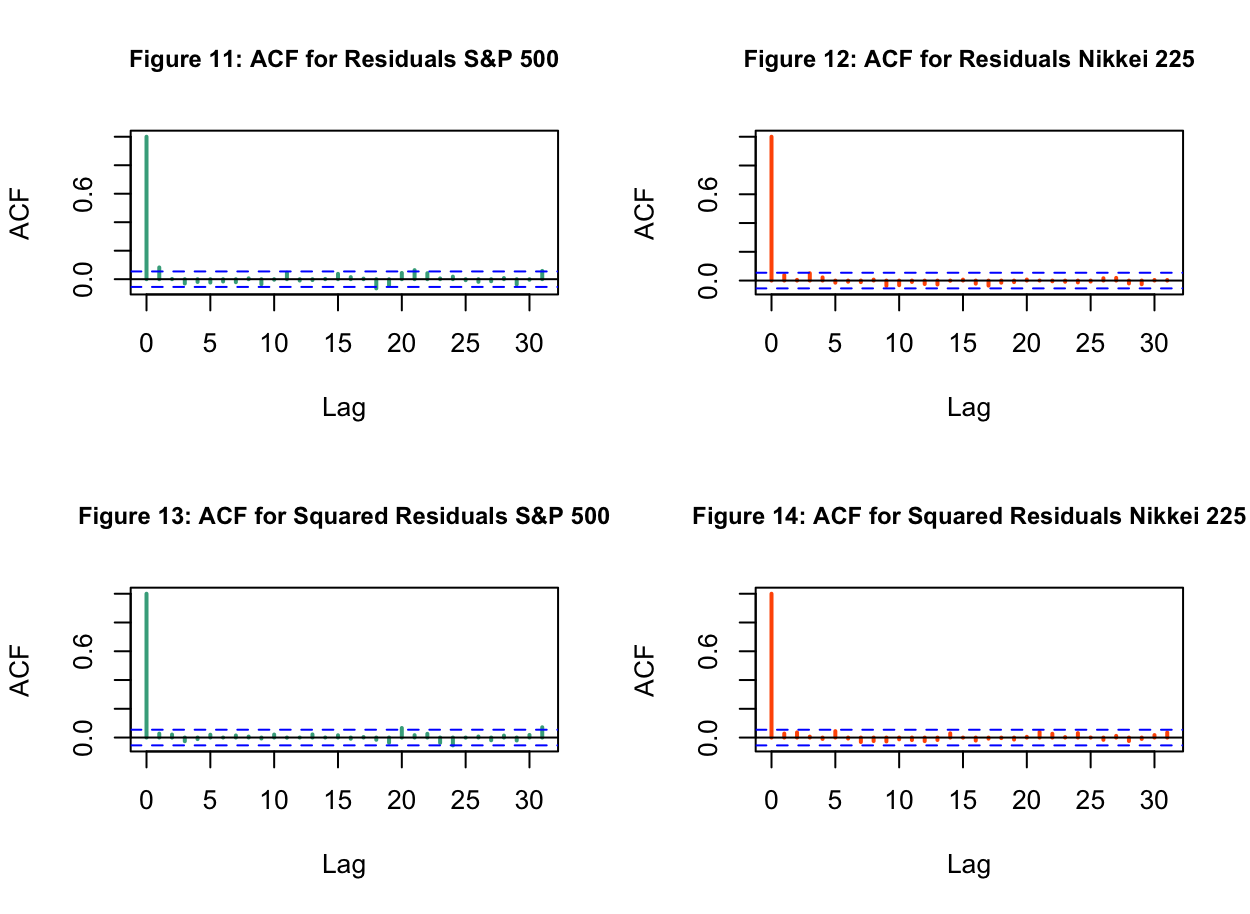
\includegraphics[width=1\linewidth]{Figure11-14.png}
    \label{fig:enter-label}
\end{figure}


\begin{figure}[htb]
    \centering
    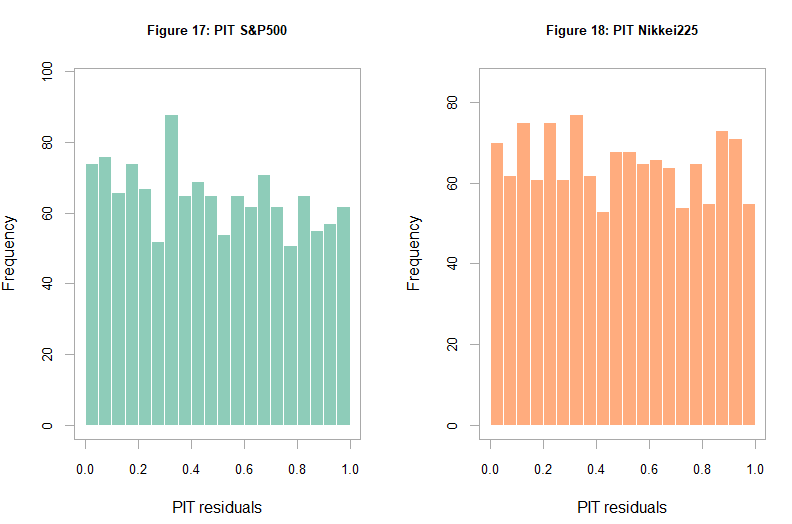
\includegraphics[width=1\linewidth]{PIT.png}
\end{figure}
\begin{figure}[htb]
    \centering
    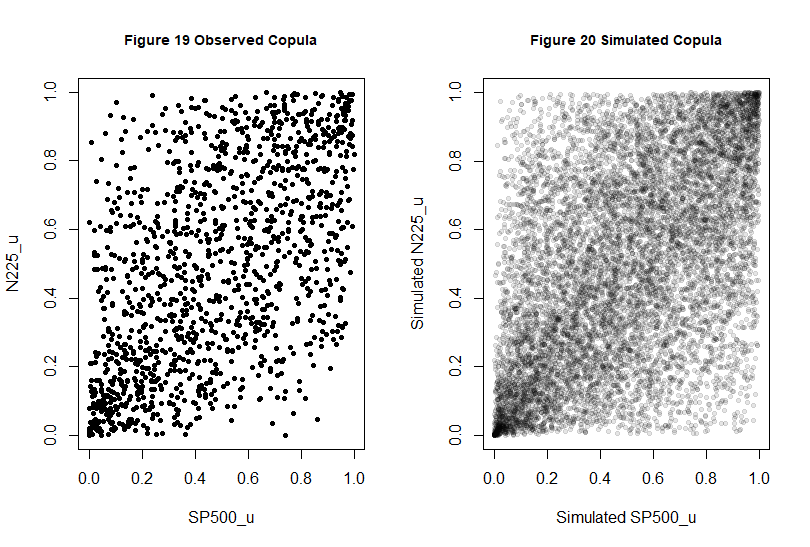
\includegraphics[width=1\linewidth]{MC sim.png}
\end{figure}

\begin{figure}[htb]
    \centering
    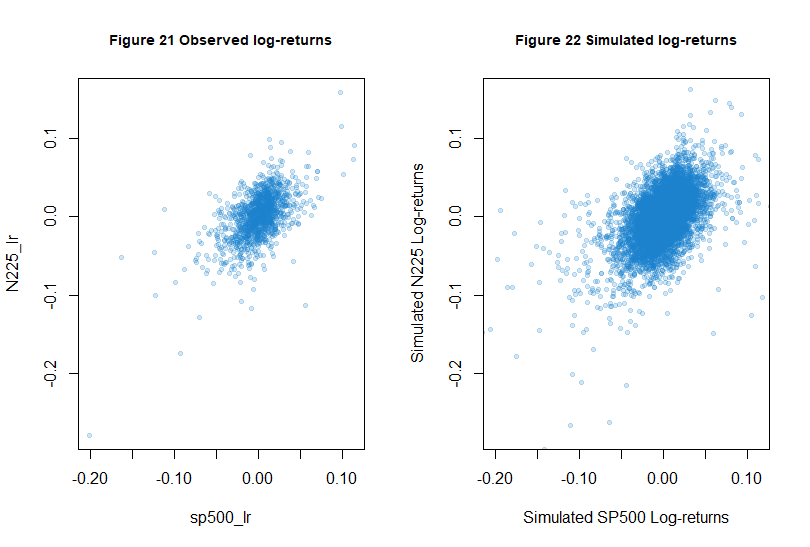
\includegraphics[width=1\linewidth]{Inverse.png}
\end{figure}

\clearpage 

\begin{table}[h!]
\centering
    \caption{Descriptive Statistics of Weekly Log-Returns of S\&P 500 and Nikkei 225}
    \begin{tabular}{lccccccc}
        \hline
        Index & Min. & Max. & Mean & Std. Dev. & Skewness & Kurtosis & Jarque-Bera Test (p-value) \\ 
        \hline
        S\&P 500 & -0.201 & 0.114 & 0.00110 & 0.025 & -0.873 & 7.192 & 0.000 \\
        Nikkei 225 & -0.279 & 0.158 & 0.00059 & 0.030 & -0.922 & 7.652 & 0.000 \\
        \hline
    \end{tabular}
    \label{table:descriptive_stats}
\end{table}

\begin{table}[h!]
    \centering
    \caption{Ljung-Box Test P-values for the Two Indices}
    \vspace{0.5cm}
    \begin{tabular}{lccccccc}
        \hline
        Index & Residuals & Squared Residuals \\ 
        \hline
        S\&P 500 & 0.125 & 0.386\\
        Nikkei 225 & 0.947 & 0.561 \\
        \hline
    \end{tabular}
\end{table}

\begin{table}[h!]
    \centering
    \caption{Monte Carlo Simulation Value-at-Risk} 
    \vspace{0.5cm}
    \begin{tabular}{lcc}
        \hline
        99\% VaR	 & 95\% VaR\\ 
        \hline
        0.07469	& 0.03707 \\
        \hline
    \end{tabular}
    \label{table:VaR}
\end{table}

\end{document}

